\section{Image processing}

\begin{frame}{Datasets} 
	\begin{itemize}
		\item Modified National Institute of Standards and Technology - MNIST (60k/10k)
		\item Canadian Institute For Advanced Research -  CIFAR-10 (50k/10k) and CIFAR-100 (2 level, 500/100) 
		\item Pascal Visual Object Classes (VOC) - 22k images, 20 classes
		\item $\dots$ 
		\item ImageNet 
	\end{itemize}
\end{frame}

\begin{frame}{ImageNet Large Scale Visual Recognition Challenge}
	\begin{columns}
		\begin{column}{.5\textwidth}
			\begin{center}
				MNIST Dataset (60k, 10k)
			\end{center}
		\end{column}
		\begin{column}{.5\textwidth}
			\begin{center}
				ImageNet (14M+, 22k)
			\end{center}
		\end{column}
	\end{columns}
	\begin{columns}
		\begin{column}{.5\textwidth}
			\begin{figure}
				\includegraphics[width=1\textwidth, center]{figures/MnistExamples}
				\caption*{}
			\end{figure}
		\end{column}
		\begin{column}{.5\textwidth}
			\begin{figure}
			\includegraphics[width=.8\textwidth, center]{figures/Examples-in-the-ImageNet-dataset}
			\caption*{}
		\end{figure}
		\end{column}
	\end{columns}
\end{frame}

\begin{frame}{ImageNet Large Scale Visual Recognition Challenge}
	\begin{columns}
		\begin{column}{.5\textwidth}
			\begin{itemize}
				\item Publicly available dataset - ImageNet (14M+, 22k categories)
				\item Annual competition 
				\begin{itemize}
					\item[-] Image classification 
					\item[-] Object detection and localization
				\end{itemize}
				\item Increasing depth 
				\begin{itemize}
					\item[-] 8 layer AlexNet
					\item[-] 19 layer  GoogLeNet
					\item[-] 152 layer ResNet 
				\end{itemize}
				
			\end{itemize}
		\end{column}
		\begin{column}{.5\textwidth}
			\begin{figure}
				\includegraphics[width=1.2\textwidth, center]{figures/ilsvrc_2015_plot}
				\caption*{Top 5 classification error rate}
			\end{figure}
		\end{column}
	\end{columns}
\end{frame}

\begin{frame}{Using linear layer}
\begin{columns}
	\begin{column}{.7\textwidth}
		\begin{block}{Image as 2D Tensor(Matrix)}
			\begin{center}
			\begin{tabular}{|c|c|c|c|c|}
				\hline
				1 & 2 & 3 & 4 & 5 \\
				\hline
				6 & 7 & 8 & 9 & 10 \\
				\hline
				5 & 4 & 3 & 2 & 1 \\
				\hline
				10 & 9 & 8& 7 & 6 \\
				\hline
			\end{tabular}
			\end{center}
		\end{block}
	\end{column}
	\begin{column}{.3\textwidth}
		\begin{block}{2D $\rightarrow$ 1D}
			\begin{tiny}
				\begin{math}
				\mathbb{W}_{m \times 20} 
				\begin{bmatrix}
				1 \\ 2 \\ 3 \\ 4 \\ 5 \\ 6 \\
				\dots \\
				8 \\ 7\\ 6 \\
				\end{bmatrix} 
				+ \mathbb{B}_{m\times 1}
				\end{math}			
			\end{tiny}
		\end{block}
	\end{column}
\end{columns}
\end{frame}

\begin{frame}{2D Convolution Example}
	\begin{figure}
		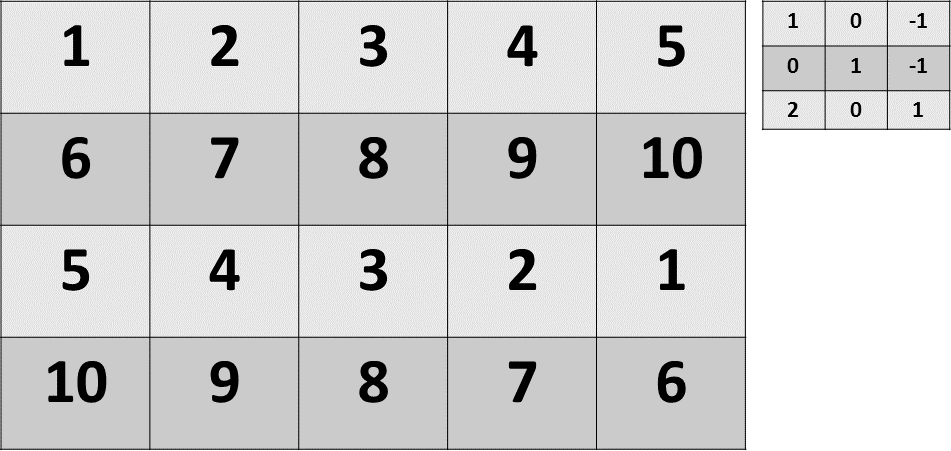
\includegraphics[width=.7\textwidth, center]{figures/conv-slide1-cropped}
	\end{figure}
\end{frame}

\begin{frame}{2D Convolution Example}
	\begin{figure}
		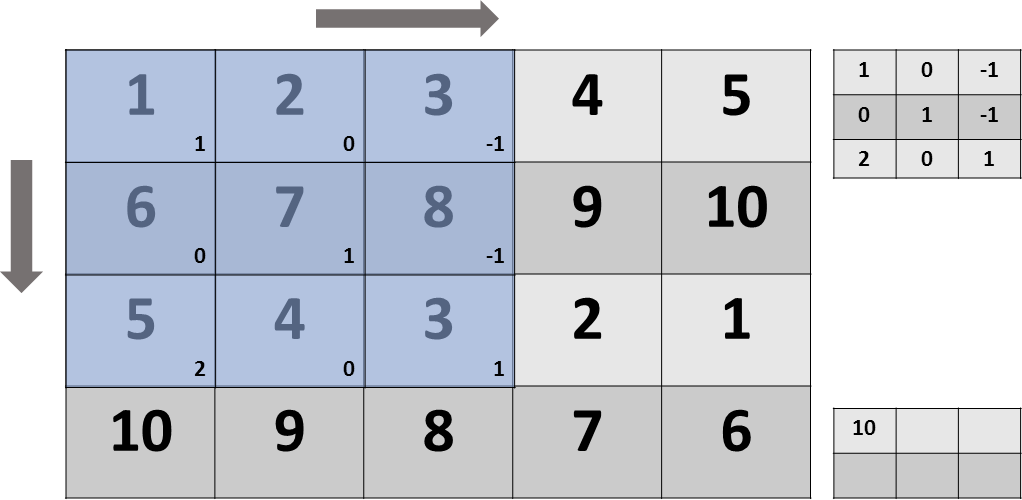
\includegraphics[width=.7\textwidth, center]{figures/conv-slide2-cropped}
	\end{figure}
	\begin{align*}
		(1\times 1)+(2\times 0)+(3\times-1)+ \\
	(6\times 0) + (7 \times 1) + (8 \times -1)+ \\
	(5\times 2) + (4\times 0) + (3\times 1)  
	\end{align*}

\end{frame}

\begin{frame}{2D Convolution Example}
	\begin{figure}
		\includegraphics[width=.7\textwidth, center]{figures/conv-slide3-cropped}
	\end{figure}
\end{frame}

\begin{frame}{2D Convolution Example}
	\begin{figure}
		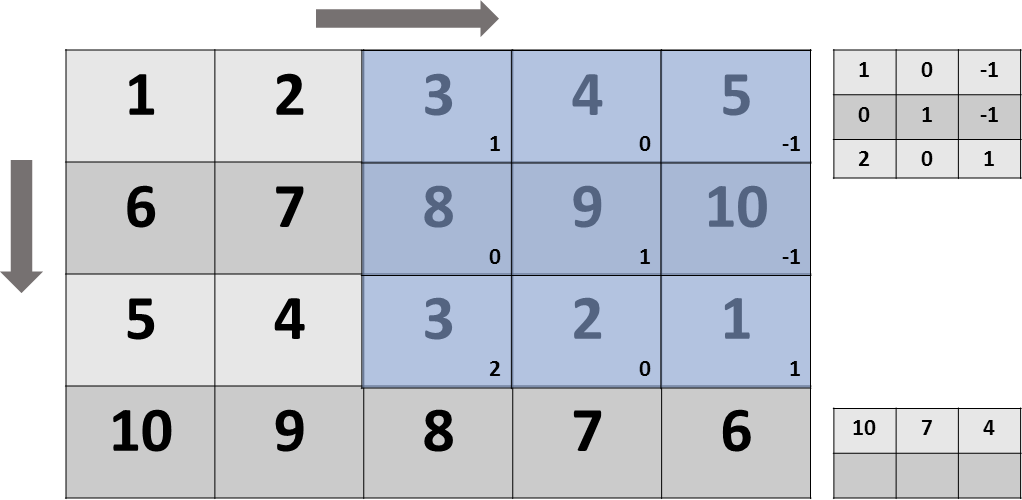
\includegraphics[width=.7\textwidth, center]{figures/conv-slide4-cropped}
	\end{figure}
\end{frame}

\begin{frame}{2D Convolution Example}
	\begin{figure}
		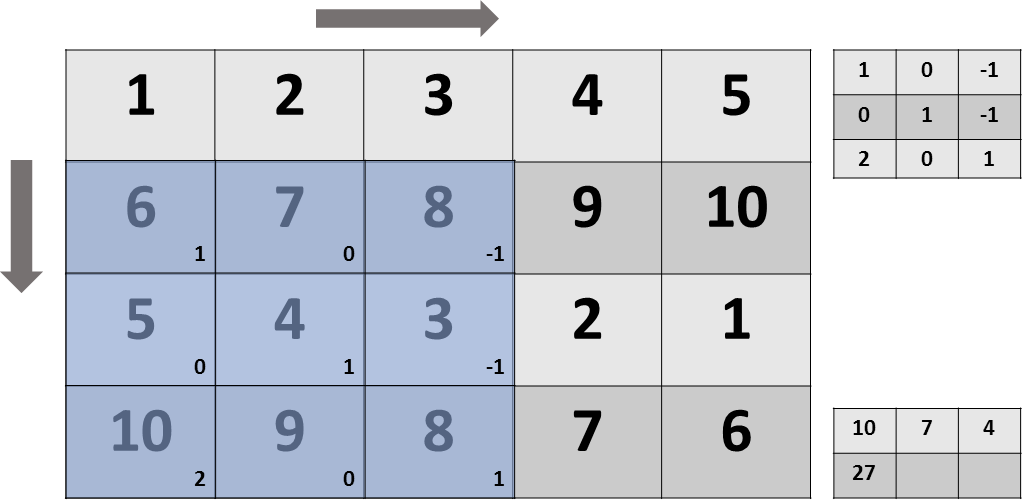
\includegraphics[width=.7\textwidth, center]{figures/conv-slide5-cropped}
	\end{figure}
\end{frame}

\begin{frame}{2D Convolution} 
	\begin{itemize}
		\item Bias $wx+b$ 
		\item Stride 
		\item Padding 
		\item Layers or channels 
	\end{itemize}
	For a $5\times5$ filter with bias, you need $26$ parameters for gray scale images. 
	If you have 3 channels (rgb), you need $5\times 5\times 3+1=76$ parameters. 
	
	
	Layers typically have multiple filters, each filter resulting in a single output channel. 
	Hence, a layer with 200 $5\times5$ filters (with bias) for 3 channel inputs  
	will have $76\times200=15,200$ parameters. Corresponding output will contain 200 channels. 
\end{frame}

\begin{frame}{Max pooling}
	\begin{figure}
			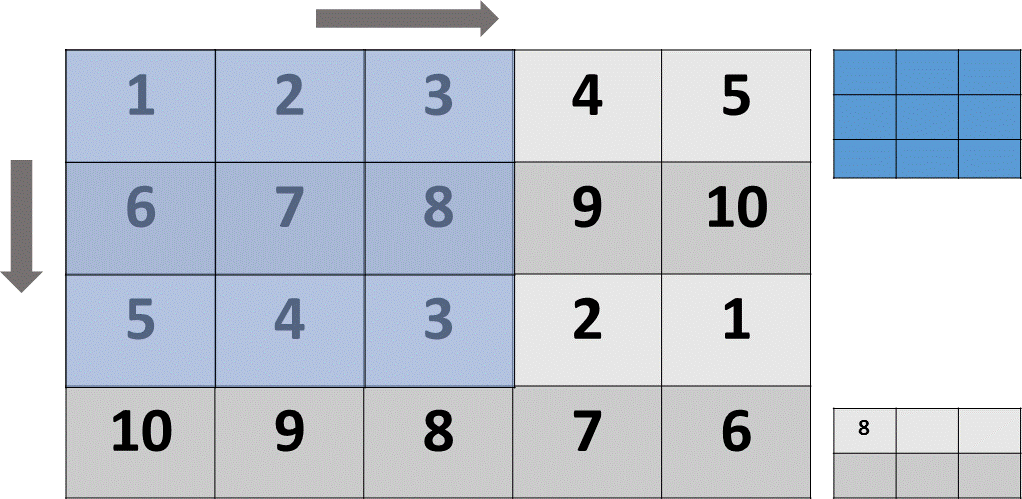
\includegraphics[width=.7\textwidth, center]{figures/maxpool2}
	\end{figure}
\end{frame}
\begin{frame}{Max pooling}
	\begin{figure}
		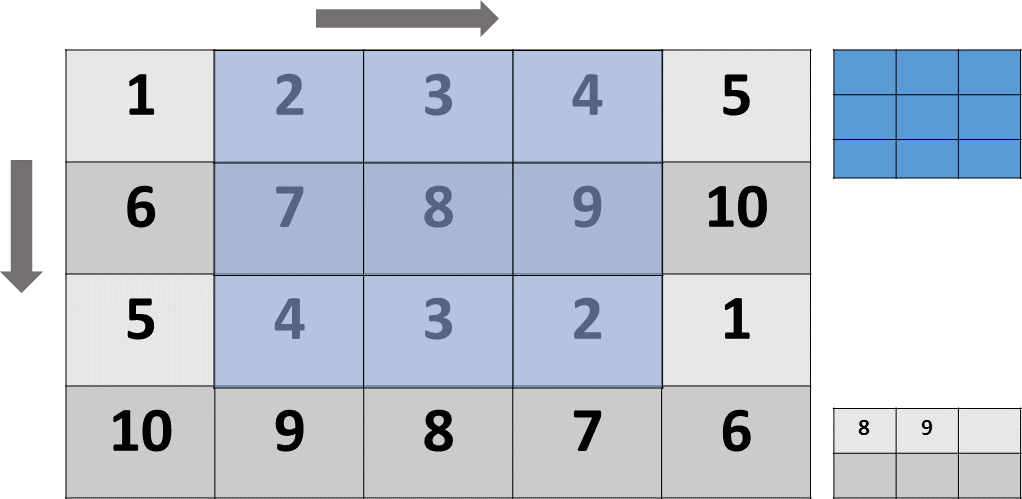
\includegraphics[width=.7\textwidth, center]{figures/maxpool3}
	\end{figure}
\end{frame}
\begin{frame}{Max pooling}
	\begin{figure}
		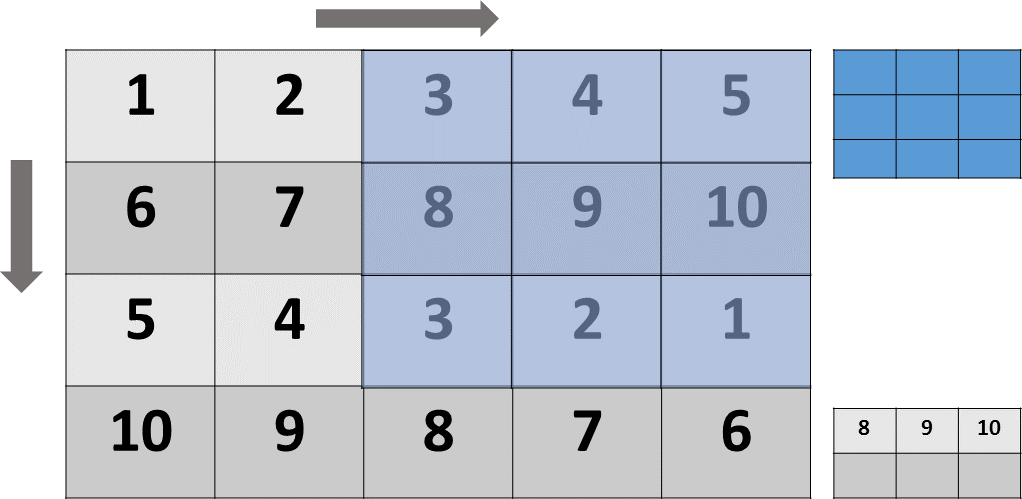
\includegraphics[width=.7\textwidth, center]{figures/maxpool4}
	\end{figure}
\end{frame}
\begin{frame}{Max pooling}
	\begin{figure}
		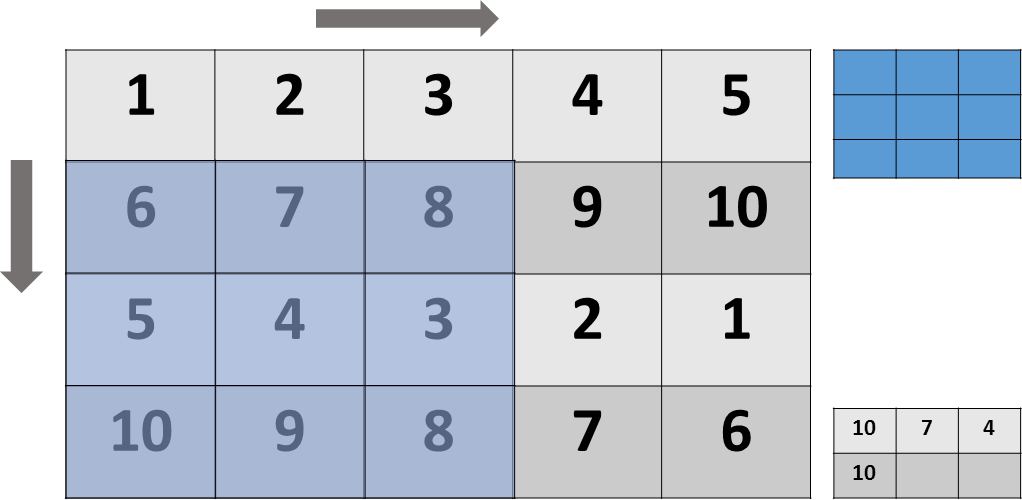
\includegraphics[width=.7\textwidth, center]{figures/maxpool5}
	\end{figure}
\end{frame}
\begin{frame}{Max pooling}
	\begin{figure}
		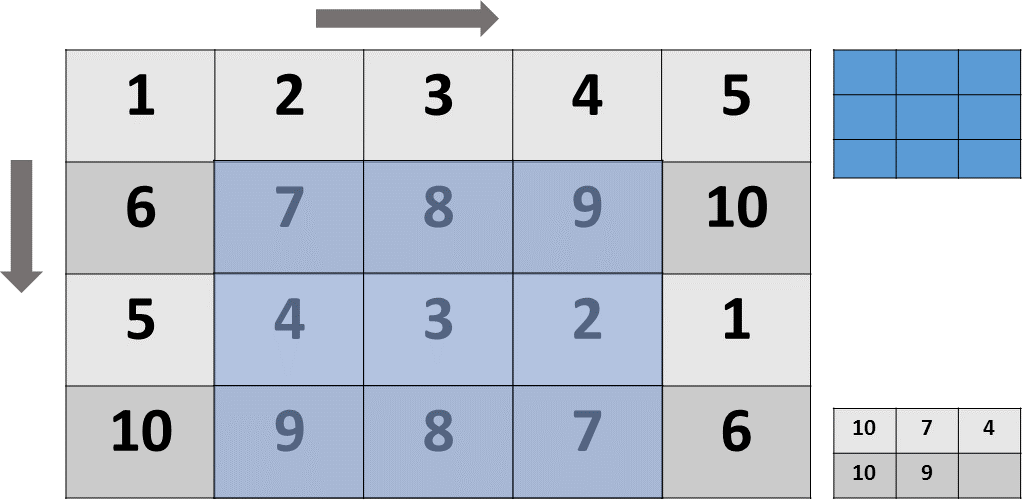
\includegraphics[width=.7\textwidth, center]{figures/maxpool6}
	\end{figure}
\end{frame}
\begin{frame}{Max pooling}
	\begin{figure}
		\includegraphics[width=.7\textwidth, center]{figures/maxpool7}
	\end{figure}
\end{frame}

\begin{frame}{Image processing}
	\begin{columns}
		\begin{column}{.5\textwidth}
			\begin{block}{Other functions}
				\begin{itemize}
					\item RelU activation: $max(x,0)$ 
					\item Leaky RelU 
					\[
					f(x;.1)= 
					\begin{cases}
					x,& \text{if } x\geq 0\\
					.1x,              & \text{otherwise}
					\end{cases}
					\] 
					\item Dropout layer 
				\end{itemize}
				\begin{figure}
					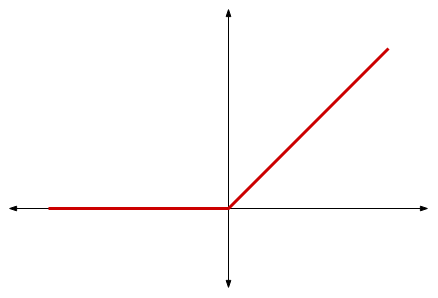
\includegraphics[width=.3\textwidth]{figures/relu}
					\caption*{\tiny{RelU}}
				\end{figure}
			\end{block}
		\end{column}
		\begin{column}{.5\textwidth}
			\begin{block}{AlexNet 2012}
				\begin{itemize}
					\item 8 Layers, 5 Convolutional, 3 fully connected
					\item Used RelU and max-pooling
					\item 61M parameters
				\end{itemize}
			\end{block}
		\end{column}
	\end{columns}

\end{frame}

\begin{frame}{AlexNet 2012}
	\begin{figure}
		\includegraphics[width=.9\textwidth, center]{figures/alexnet-arch}
		\caption*{Alex Krizhevsky, Sutskever, Ilya and Hinton, Geoffrey E., "ImageNet Classification with Deep Convolutional Neural Networks", 2012 }
	\end{figure}
\end{frame}
\begin{frame}{Typical convolution net, pytorch}
	\begin{lstlisting}[language=Python,caption={Typical (simple) CNN in pytorch}]
class ConvNet(nn.Module):
  def __init__(self):
    super(ConvNet, self).__init__()
    self.conv1 = nn.Conv2d(3, 16, 3, padding=1) 
    self.lrelu1 = nn.LeakyReLU(.1) 
    self.conv2 = nn.Conv2d(16, 32, kernel_size=3, padding=1)
    self.lrelu2 = nn.LeakyReLU(.1) 
    self.maxpool1 = nn.MaxPool2d(kernel_size=3, padding=1)
    self.dropout1 = nn.Dropout(p=.25)
    self.conv3 = nn.Conv2d(in_channels=32, out_channels=32, padding=1, kernel_size=3)
    self.lrelu2 = nn.LeakyReLU(0.1)
    self.conv4 = nn.Conv2d(in_channels=32, out_channels=64, padding=1, kernel_size=3)
    self.lrelu3 = nn.LeakyReLU(0.1)
    self.maxpool2 = nn.MaxPool2d(kernel_size=3, padding=1)
    self.dropout2 = nn.Dropout(p=.25)
    
    self.conv_layers = [self.conv1, self.lrelu1, self.conv2, self.lrelu2, self.maxpool1, self.dropout1, 
    self.conv3, self.lrelu2, self.conv4, self.lrelu3, self.maxpool2, self.dropout2]
    
    self.fc1 = nn.Linear(in_features=64*4*4, out_features=256)
    self.lrelu4 = nn.LeakyReLU(.1)
    self.dropout3 = nn.Dropout(.25) 
    self.fc2 = nn.Linear(in_features=256, out_features=10)
    self.softmax = nn.Softmax(dim=1) 
    
    self.flat_layers  = [self.fc1, self.lrelu4, self.dropout3, self.fc2, self.softmax]
\end{lstlisting}

\end{frame}


